\documentclass[letterpaper]{article}
\usepackage[submission]{aaai2027}
\usepackage[hyphens]{url}
\usepackage{graphicx}
\urlstyle{rm}
\def\UrlFont{\rm}
\usepackage{natbib}
\usepackage{caption}
\frenchspacing

\usepackage{amsmath}
\usepackage{amssymb}
\usepackage{array}
\usepackage{booktabs}

\pdfinfo{
/TemplateVersion (2027.1)
}

\setcounter{secnumdepth}{0}

\title{Adaptive Proximal Control for Federated Personalization\\Supplementary Material}

\author{
    Anonymous Submission
}
\affiliations{
}

\begin{document}

\maketitle

\section{Experimental Protocol}

Tables~\ref{tab:supp-protocol} and~\ref{tab:supp-sweep-protocol}
give the protocol details behind the main-paper figures.

\section{Controller Details}

Adaptive proximal control replaces a fixed proximal coefficient with a
bounded client-side control state. We refer to the FedProx instantiation
as AdaFedProx and the Ditto instantiation as AdaDitto. For FedProx, this
state is $\mu_i^{(t)}$; for Ditto, it is $\lambda_i^{(t)}$.

At the start of round $t$, the server broadcasts $w^{(t)}$ and the
previous reference $L_g^{(t-1)}$. Client $i$ evaluates the received
global model on a local probe minibatch and obtains $\hat L_i^{(t)}$.
The minibatch is taken from the shuffled local training loader before
local optimization, using 10\% of local training examples capped at
256 examples, with at least one example. The probe uses inference mode
and no gradients. The client computes
\[
g_i^{(t)}=\mathrm{clip}\left(\log\frac{\hat L_i^{(t)}+\epsilon}{L_g^{(t-1)}+\epsilon},0,\tau\right).
\]
For AdaDitto, the coefficient target is
$\lambda_{\mathrm{base}}+\alpha g_i^{(t)}$, then smoothed with rate
$\gamma$ and clipped to $[\lambda_{\min},\lambda_{\max}]$. AdaFedProx
uses the analogous $\mu$ notation. The resulting coefficient is used in
the ordinary FedProx or Ditto proximal objective for that client's local
update. The client returns its model update and scalar probe loss, and
the server updates the reference for future rounds using a median
exponential moving average over the returned probe losses. The main
paper lists the default AdaDitto values; the sensitivity scans below
vary them around that default.

The controller does not change aggregation or the underlying FedProx and
Ditto objectives beyond replacing a static coefficient with a controlled
one. It preserves the model-update communication pattern and adds one
scalar loss report per participating client and one scalar reference in
the server broadcast.

\section{Controller Trajectories}

Figure~\ref{fig:supp-controller-trajectories} shows that the adaptive
coefficient changes smoothly rather than jumping to extreme values. The
controller increases coupling under both CIFAR-pathological partial
participation and Shakespeare, but settles in different ranges.

\begin{figure*}[t]
  \centering
  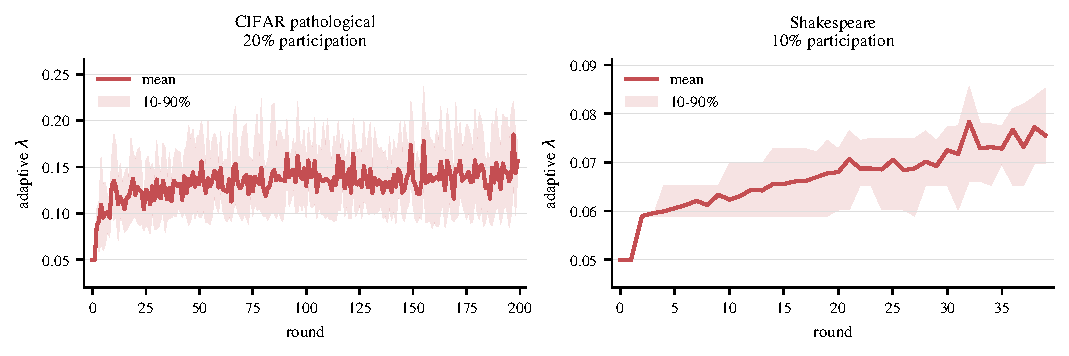
\includegraphics[width=0.95\textwidth]{Figures/current/controller_trajectories.pdf}
  \caption{Adaptive Ditto coefficient trajectories. Lines show the mean coefficient over participating clients and seeds; bands show the 10th--90th percentile range.}
  \label{fig:supp-controller-trajectories}
\end{figure*}

\section{Controller Signal Validity}

We audited whether the controller's loss-gap signal tracks the anchoring
need rather than merely producing a plausible coefficient trajectory.
Table~\ref{tab:signal-validity} reports post-warmup averages over
participating clients: the clipped log loss-gap $g_i$, the fraction of
positive gaps, and the learned final Ditto coefficient.

Within a run, the raw controller target is affine in the loss gap by
construction, so the target-gap correlation checks implementation rather
than mechanism. The cross-condition comparison is the relevant signal:
on both CIFAR splits, 20\% participation yields much larger gaps than
full participation and correspondingly larger learned coefficients,
matching the known shift toward $\lambda^\star=1.0$ under partial
participation. This supports a mechanistic reading of the CIFAR shift
result: the controller increases anchoring where the loss-gap signal
says anchoring is needed.

The same audit also identifies a real limitation. The lower coefficient
bound is load-bearing. When the known optimum is near zero, as in
CIFAR-pathological full participation, AdaDitto cannot reach zero and
slightly over-anchors. On Shakespeare, the loss gap is nearly zero, so
AdaDitto's parity with tuned Ditto appears to come mainly from the
lower-bound floor rather than active gap-driven adaptation. This does
not weaken the CIFAR participation-shift mechanism, but it scopes the
controller: the gap is informative under CIFAR participation shift,
while the floor acts as a safety net when the signal is weak.

\section{Controller Sensitivity}

We scanned 28 AdaDitto controller configurations on CIFAR-100 practical,
varying gain, smoothing, EMA behavior, clipping threshold, and maximum
coefficient. Final personalized accuracy ranged from 0.4762 to 0.4791,
a spread of 0.29 points. The default configuration was tied-best
(Table~\ref{tab:controller-scan}).

We also ran an 11-configuration stress scan at the two headline
conditions: CIFAR-100 pathological with 20\% participation and
Shakespeare with 10\% participation. Table~\ref{tab:headline-controller-scan}
reports the sorted-scan summary. On CIFAR-pathological, every
controller configuration remains above the stale tune-once baseline and
the default is median-ranked. On Shakespeare, the three-seed scan lies
within 0.03 points and remains within 0.13 points of the tuned
fixed-Ditto optimum. These scans test whether the headline results
depend on a lucky default controller setting; they do not.

We also ablated controller mechanisms across both CIFAR splits. On the
practical split, all modes were close relative to seed variation, so the
random-adaptive row should not be read as a mechanism improvement. It
is kept only as a sanity check: on the pathological split, principled
modes clustered around 0.597, while random adaptive coefficients fell
to 0.5863 (Table~\ref{tab:controller-ablations}).

\section{Tune-Once Regret Matrix}

Table~\ref{tab:tune-once-regret} reframes coefficient brittleness as
deployment regret. Each target column has its own best fixed $\lambda$
on the common CIFAR grid. Static rows select $\lambda$ in the source
condition and deploy that same value unchanged on each target.

A fixed $\lambda$ is safe only when the deployment condition resembles
the tuning condition. The $\lambda=0$ setting selected by
CIFAR-pathological under high participation is optimal there, but loses
4.7 points on pathological 20\% participation and 7.2 points on
practical 20\% participation. AdaDitto does not match the per-condition
oracle, but its observed regret is bounded by 3.2 points across the
same targets. Thus the controller acts as a downside cap rather than an
oracle replacement.

\section{FedProx Negative Probe}

FedProx's proximal term did not improve CIFAR-100 in the tested
regimes. This explains why AdaFedProx is mostly a parity result: when
the best $\mu$ is approximately zero, there is no useful proximal signal
for an adaptive $\mu$ controller to recover. Table~\ref{tab:fedprox-null}
summarizes the negative probe.

\section{Shakespeare Details}

Shakespeare supplies the text-modality check. Its optimal direction
differs from CIFAR-pathological: pure-local Ditto is poor, while
nonzero coupling is essential. Table~\ref{tab:shakespeare-sweep} shows
that the best fixed coefficient remains stable across the tested
participation levels, and Table~\ref{tab:shakespeare-core} shows that
AdaDitto matches tuned Ditto rather than producing a shift win.

\section{Reproducibility Details}
\label{app:reproducibility}

Tables~\ref{tab:reproducibility-details} and~\ref{tab:final-hyperparameters}
summarize implementation, data, hardware, randomness, reporting, and
final training hyperparameters.

\begin{table*}[t]
\centering
\scriptsize
\setlength{\tabcolsep}{3pt}
\renewcommand{\arraystretch}{1.08}
\begin{tabular*}{\textwidth}{@{\extracolsep{\fill}}lrlp{0.20\textwidth}lrrp{0.22\textwidth}@{}}
\toprule
\textbf{Dataset} & \textbf{Clients} & \textbf{Model} & \textbf{Partition} & \textbf{Participation} & \textbf{Rounds} & \textbf{Rep.} & \textbf{Role} \\
\midrule
CIFAR-100 practical & 20 & CNN & Dirichlet $\alpha=0.1$, overlapping labels & full, 50\%, 20\% & 200 & mixed & fixed sweeps, core comparisons, controller scans \\
CIFAR-100 pathological & 20 & CNN & label shards, 10 labels/client & full, 50\%, 20\% & 200 & mixed & fixed sweeps, tune-once shift, core comparisons \\
Shakespeare & 118 & char-LSTM & LEAF speakers & 10\%, 50\% & 40 & mixed & fixed sweeps, text-modality and controller checks \\
\bottomrule
\end{tabular*}
\caption{Experimental protocol. Main-paper figures report outcome comparisons; replication counts are mixed by experiment role and specified in Table~\ref{tab:supp-sweep-protocol}.}
\label{tab:supp-protocol}
\end{table*}

\begin{table*}[t]
\centering
\scriptsize
\setlength{\tabcolsep}{4pt}
\renewcommand{\arraystretch}{1.08}
\begin{tabular*}{\textwidth}{@{\extracolsep{\fill}}p{0.26\textwidth}p{0.54\textwidth}p{0.14\textwidth}@{}}
\toprule
\textbf{Experiment role} & \textbf{Grid or comparison rule} & \textbf{Replication} \\
\midrule
CIFAR full-participation sweeps &
$\lambda\in\{0,10^{-3},0.005,10^{-2},0.03,0.05,0.08,0.1,0.2,0.5,1,2,3\}$ &
one seed \\
CIFAR partial-participation sweeps &
$\lambda\in\{0,10^{-3},10^{-2},0.1,0.5,1\}$ &
one seed \\
Shakespeare fixed-Ditto sweeps &
$\lambda\in\{0,0.1,0.5,1\}$ at 10\% and 50\% participation &
one seed \\
Tune-once shift tests &
Select the full-participation fixed $\lambda$, freeze it, and reuse it under shifted participation without retuning &
three seeds \\
CIFAR per-condition core comparisons &
Re-sweep static Ditto for each dataset and participation level before comparing against AdaDitto &
five seeds \\
Controller sensitivity scans &
Vary AdaDitto controller configurations around the default: 28 configurations on CIFAR-100 practical and 11 configurations at each headline condition &
three seeds for reported stress scans \\
\bottomrule
\end{tabular*}
\caption{Sweep grids and replication rules. Single-seed sweeps identify coefficient regimes; multi-seed comparisons estimate robustness for the main claims.}
\label{tab:supp-sweep-protocol}
\end{table*}

\begin{table*}[t]
\centering
\small
\setlength{\tabcolsep}{8pt}
\renewcommand{\arraystretch}{1.08}
\begin{tabular*}{\textwidth}{@{\extracolsep{\fill}}lcccc@{}}
\toprule
\textbf{Condition} & $\boldsymbol{\lambda^\star}$ & \textbf{Mean gap} & \textbf{Gap $>$ 0} & \textbf{Learned $\lambda$} \\
\midrule
CIFAR-path full & 0.0 & 0.013 & 33\% & 0.090 \\
CIFAR-path 20\% & 1.0 & 0.074 & 52\% & 0.135 \\
CIFAR-prac full & 0.5 & 0.008 & 30\% & 0.086 \\
CIFAR-prac 20\% & 1.0 & 0.030 & 46\% & 0.101 \\
Shakespeare 10\% & $>0$ & 0.003 & 5\% & 0.069 \\
\bottomrule
\end{tabular*}
\caption{Controller signal-validity audit. The CIFAR participation-shift rows show larger loss gaps and larger learned coefficients exactly where the best fixed $\lambda$ moves upward.}
\label{tab:signal-validity}
\end{table*}

\begin{table*}[t]
\centering
\small
\setlength{\tabcolsep}{8pt}
\renewcommand{\arraystretch}{1.08}
\begin{tabular*}{\textwidth}{@{\extracolsep{\fill}}lcc@{}}
\toprule
\textbf{Setting} & \textbf{Accuracy range} & \textbf{Spread} \\
\midrule
AdaDitto controller scan & 0.4762--0.4791 & 0.0029 \\
\bottomrule
\end{tabular*}
\caption{CIFAR-100 practical controller scan over 28 configurations.}
\label{tab:controller-scan}
\end{table*}

\begin{table*}[t]
\centering
\small
\setlength{\tabcolsep}{8pt}
\renewcommand{\arraystretch}{1.08}
\begin{tabular*}{\textwidth}{@{\extracolsep{\fill}}lcc@{}}
\toprule
\textbf{Quantity} & \textbf{CIFAR-path 20\%} & \textbf{Shakespeare 10\%} \\
\midrule
Seeds & 3 & 3 \\
Configs & 11 & 11 \\
Accuracy range & 0.5627--0.5743 & 0.4819--0.4822 \\
Spread & 1.2 points & 0.03 points \\
Default rank & 6/11 & 5/11 \\
Reference & tune-once 0.551 & tuned 0.483 \\
Outcome & all beat tune-once & all near tuned \\
Coeff. mean range & 0.087--0.190 & 0.055--0.085 \\
\bottomrule
\end{tabular*}
\caption{Controller stress scans at the headline conditions. Both scans use three seeds per controller configuration and test whether the headline results depend on a lucky default controller setting.}
\label{tab:headline-controller-scan}
\end{table*}

\begin{table*}[t]
\centering
\small
\setlength{\tabcolsep}{8pt}
\renewcommand{\arraystretch}{1.08}
\begin{tabular*}{\textwidth}{@{\extracolsep{\fill}}lcc@{}}
\toprule
\textbf{Mode} & \textbf{Practical} & \textbf{Pathological} \\
\midrule
full controller & 0.4689 & 0.5968 \\
fixed base & 0.4677 & 0.5976 \\
no log ratio & 0.4685 & 0.5971 \\
no clipping & 0.4689 & 0.5968 \\
no EMA & 0.4693 & 0.5971 \\
mean reference loss & 0.4681 & 0.5974 \\
global shared coefficient & 0.4657 & 0.5967 \\
random adaptive & 0.4768 & 0.5863 \\
\bottomrule
\end{tabular*}
\caption{Mean personalized accuracy for controller ablations over three seeds. The random-adaptive row is a negative-control sanity check; its practical-split value is not interpreted because all practical modes are close to seed variation, while it clearly hurts under high heterogeneity.}
\label{tab:controller-ablations}
\end{table*}

\begin{table*}[t]
\centering
\small
\setlength{\tabcolsep}{8pt}
\renewcommand{\arraystretch}{1.08}
\begin{tabular*}{\textwidth}{@{\extracolsep{\fill}}lcccc@{}}
\toprule
\textbf{Tuned source} & $\boldsymbol{\lambda}$ &
\textbf{1.0} & \textbf{0.5} & \textbf{0.2} \\
\midrule
\multicolumn{5}{l}{\textbf{Practical targets}} \\
prac/1.0, prac/0.5 & 0.5 & 0.000 & 0.000 & 0.003 \\
prac/0.2, path/0.2 & 1.0 & 0.002 & 0.000 & 0.000 \\
path/1.0, path/0.5 & 0.0 & 0.025 & 0.033 & 0.072 \\
\midrule
AdaDitto, one config & -- & 0.017 & 0.021 & 0.032 \\
\midrule
\multicolumn{5}{l}{\textbf{Pathological targets}} \\
prac/1.0, prac/0.5 & 0.5 & 0.022 & 0.008 & 0.003 \\
prac/0.2, path/0.2 & 1.0 & 0.026 & 0.010 & 0.000 \\
path/1.0, path/0.5 & 0.0 & 0.000 & 0.000 & 0.047 \\
\midrule
AdaDitto, one config & -- & 0.024 & 0.017 & 0.023 \\
\bottomrule
\end{tabular*}
\caption{Tune-once regret on CIFAR-100. Columns show target participation. Each cell reports accuracy lost relative to the target condition's best fixed $\lambda$ on the common grid $\{0,0.001,0.01,0.1,0.5,1.0\}$. Fixed-$\lambda$ sweep cells are single-seed diagnostics, so small differences should be interpreted cautiously; the large 4.7--7.2 point failures are the relevant signal.}
\label{tab:tune-once-regret}
\end{table*}

\begin{table*}[t]
\centering
\small
\setlength{\tabcolsep}{8pt}
\renewcommand{\arraystretch}{1.08}
\begin{tabular*}{\textwidth}{@{\extracolsep{\fill}}p{0.48\textwidth}p{0.42\textwidth}@{}}
\toprule
\textbf{Regime} & \textbf{Outcome} \\
\midrule
E=1, full participation & small or zero $\mu$ best \\
E=5, full participation & $\mu=0$: 0.635; $\mu=1.0$: 0.571 \\
E=5, 20\% participation & $\mu=0$: 0.230; $\mu>0$: 0.196 \\
E=5, 20\% with systems heterogeneity & $\mu=0$: 0.259; $\mu=1.0$: 0.222 \\
\bottomrule
\end{tabular*}
\caption{FedProx $\mu$ probes on CIFAR-100. Larger proximal penalties did not beat FedAvg-style $\mu=0$ even under more local work and systems heterogeneity.}
\label{tab:fedprox-null}
\end{table*}

\begin{table*}[t]
\centering
\small
\setlength{\tabcolsep}{8pt}
\renewcommand{\arraystretch}{1.08}
\begin{tabular*}{\textwidth}{@{\extracolsep{\fill}}lcc@{}}
\toprule
\textbf{Fixed $\lambda$} & \textbf{10\% participation} & \textbf{50\% participation} \\
\midrule
0.0 & 0.344 & 0.445 \\
0.1 & 0.483 & 0.512 \\
0.5 & 0.483 & 0.511 \\
1.0 & 0.483 & 0.511 \\
\bottomrule
\end{tabular*}
\caption{Shakespeare fixed-Ditto sweep. Nonzero coupling is essential, and the best coefficient remains stable across the tested participation levels.}
\label{tab:shakespeare-sweep}
\end{table*}

\begin{table*}[t]
\centering
\small
\setlength{\tabcolsep}{8pt}
\renewcommand{\arraystretch}{1.08}
\begin{tabular*}{\textwidth}{@{\extracolsep{\fill}}lccc@{}}
\toprule
\textbf{Participation} & \textbf{Tuned Ditto} & \textbf{AdaDitto} & \textbf{Gap} \\
\midrule
10\% & $0.4822 \pm 0.0028$ & $0.4820 \pm 0.0029$ & -0.0001 \\
50\% & 0.5122 & 0.5118 & -0.0004 \\
\bottomrule
\end{tabular*}
\caption{Shakespeare core comparison. AdaDitto matches tuned Ditto, but there is no shift win because the optimal fixed coefficient does not move.}
\label{tab:shakespeare-core}
\end{table*}

\begin{table*}[t]
\centering
\small
\setlength{\tabcolsep}{4pt}
\renewcommand{\arraystretch}{1.08}
\begin{tabular*}{\textwidth}{@{\extracolsep{\fill}}p{0.20\textwidth}p{0.73\textwidth}@{}}
\toprule
\textbf{Item} & \textbf{Details} \\
\midrule
Datasets &
CIFAR-100~\cite{krizhevsky2009learning} and Shakespeare from the LEAF federated benchmark~\cite{caldas2018leaf}. We do not introduce new datasets. \\
Data availability &
CIFAR-100 is obtained from the public CIFAR distribution. Shakespeare is obtained through the public LEAF benchmark preprocessing pipeline. Raw datasets are not redistributed with this submission; users should follow the terms of the upstream sources. \\
Code availability &
Experiments are implemented as modifications to PFLlib~\cite{zhang2025pfllib}. An anonymized code archive is provided at the URL in the main paper. Upon de-anonymization, code and experiment scripts will be released under the Apache-2.0 license inherited from the PFLlib codebase. \\
Hardware &
Run manifests for the reported phases record an NVIDIA GeForce RTX 5060 Laptop GPU. The inspection environment reports an Intel Core Ultra 7 255HX CPU exposed to WSL2 as 8 logical CPUs and 23 GiB RAM. GPU VRAM and Windows host build were not captured in the run manifests; the WSL environment is Ubuntu 24.04.4 LTS on Linux 6.6.87.2-microsoft-standard-WSL2. \\
Software &
Run manifests for the reported phases record Python 3.10.20, PyTorch 2.8.0+\texttt{cu128}, and CUDA 12.8. The active \texttt{pfllib} environment used for artifact inspection contains torchvision 0.23.0+\texttt{cu128}, NumPy 2.2.6, pandas 2.3.3, SciPy 1.15.3, h5py 3.16.0, matplotlib 3.10.8, and cuDNN 9.10.2 as reported by PyTorch. \\
Randomness and seeds &
Five-seed CIFAR core comparisons use seeds \texttt{0,1,2,3,4}. Three-seed Shakespeare core comparisons, tune-once shift runs, and controller stress scans use seeds \texttt{0,1,2}. Single-seed sweep-only configurations use seed \texttt{0}. Each run applies the seed to Python, NumPy, PyTorch CPU, and PyTorch CUDA RNGs before data partitioning, model initialization, client sampling, and minibatch shuffling; client constructors additionally seed PyTorch with \texttt{seed + client\_id}. Paired method comparisons use the same seed set. \\
Model and training hyperparameters &
Final training hyperparameters are listed in Table~\ref{tab:final-hyperparameters}. Controller hyperparameters use the default AdaDitto setting unless a sensitivity scan explicitly varies them: $\lambda_{\mathrm{base}}=0.08$, $\lambda_{\min}=0.05$, $\lambda_{\max}=3.0$, $\alpha=0.8$, $\tau=0.7$, $\gamma=0.3$, $\beta=0.9$, $\epsilon=10^{-8}$, two warmup rounds, and a 10\% probe sample capped at 256 examples. \\
Statistical reporting &
No null-hypothesis significance tests are used for the claims in the main paper. Multi-seed core comparisons report mean and standard deviation across seeds and preserve paired seed comparisons whenever methods share the same seed set. Sweep-only configurations run with a single seed are used for hyperparameter selection and sensitivity visualization, not for significance claims. \\
\bottomrule
\end{tabular*}
\caption{Reproducibility details for the experimental protocol. Values are taken from experiment scripts, run manifests, and the local environment where the artifacts were inspected; unavailable hardware fields are stated explicitly rather than inferred.}
\label{tab:reproducibility-details}
\end{table*}

\begin{table*}[t]
\centering
\small
\setlength{\tabcolsep}{4pt}
\renewcommand{\arraystretch}{1.08}
\begin{tabular*}{\textwidth}{@{\extracolsep{\fill}}p{0.18\textwidth}p{0.10\textwidth}p{0.08\textwidth}p{0.18\textwidth}p{0.10\textwidth}p{0.09\textwidth}p{0.14\textwidth}@{}}
\toprule
\textbf{Dataset} & \textbf{Model} & \textbf{Rounds} & \textbf{Clients / participation} & \textbf{Local epochs} & \textbf{Batch size} & \textbf{Optimizer / LR} \\
\midrule
CIFAR-100 practical & CNN & 200 & 20 / full, 50\%, 20\% & 1 & 64 & SGD / 0.01 \\
CIFAR-100 pathological & CNN & 200 & 20 / full, 50\%, 20\% & 1 & 64 & SGD / 0.01 \\
Shakespeare 10\% & char-LSTM & 40 & 118 / 10\% & 1 & 64 & SGD / 0.5 \\
Shakespeare 50\% & char-LSTM & 40 & 118 / 50\% & 1 & 64 & SGD / 0.5 \\
\bottomrule
\end{tabular*}
\caption{Final training hyperparameters used in the reported experiments. All rows use SGD with no weight decay. Ditto and AdaDitto train both the global and personalized models with the same local learning rate; the personalized Ditto optimizer adds the proximal step with the fixed or adaptive coefficient.}
\label{tab:final-hyperparameters}
\end{table*}

\bibliography{references}

\end{document}
